\chapter{Model and General Principles}
\label{ch:background}

This chapter will discuss the model and general principles, which serve the foundation to understand the implementation reports of the following chapter. Its important to understand every subsection of this chapter, such as the ethereum blockchain, \ac{PoW}, the \ac{EVM} and all topics needed for atmoic cross-chain swaps. 

% MB NOT HERE - - write about bitcoin and what changes it brought - buterin eth paper

%
% Section: Der erste Abschnitt
%
\section{Ethereum Blockchain}
\label{sec:background:first_section}
The Ethereum blockchain was introduced in Vitalik Buterin’s paper in 2013, which addressed several limitations of the Bitcoin’s scripting language \cite{buterin2013ethereum} based on Buterin's white paper Wood released the yellow paper one year later \cite{wood2014ethereum}. The main contributions are full Turing-completeness and saving all states of computations in between the states \cite{dannen2017introducing}.
Through its own programming language Solidity, it provides an abstract layer enabling anyone to create their own rules for ownership, formats of transactions, and state transition functions \cite{vujivcic2018blockchain}. Development was funded by an online crowdsale that took place between July and August 2014 \cite{tapscott2016blockchain}. The system then went live on 30 July 2015 \footfullcite{"Ethereum Launches" - https://blog.ethereum.org/2015/07/30/ethereum-launches/. Retrieved 30 July 2015} and is called the ethereum public blockchain. Which means its accessible to everyone who wants to send Ether token or execute smart contracts. In general we have to distinguish between private and public blockchains. The public one is described above. Since everybody can go to github and fork e.g the geth client its possible to start an own private blockchain. In an enterprise software context, where corporate stakeholders are given certain rights and privileges to read and write to the company chain, the deployment is known as a permissioned blockchain. Nevertheless for both the private (permissioned) and the public blockchain its possible to do the following \cite{dannen2017introducing}:

\begin{itemize}
	\item Send and receive Ether
	\item Write smart contracts
	\item Create provably fair applications
	\item Launch your own token based on Ether
\end{itemize}

% ADD LINEBREAK TO FOOTNOTE AND ADD THIS AT THE BEGINNING   Foundation, Ethereum 

\clearpage

\subsection{Proof-of-Work Consensus Algorithm}
\label{subsec:background:first_section:second_subsection}

%MB check wood paper for more historical PoW data!!

The \ac{PoW} system of bitcoin and ethereum is similar to Adam Back's Hashcash \cite{back2002hashcash}, but instead of a newspaper or Usenet post the \ac{PoW} involves scanning for a value, which is hashed with the \ac{SHA-256} to begin with a number of zero bits. The average work required is exponential. Which means the more leading zeros, the more work. In the end the work can be later verified by executing a single hash. The \ac{PoW} is implemented by incrementing a nonce in the block until a value is found that gives the block's hash the required zero bits. The majority decision is represented by the longest chain, which has the greatest \ac{PoW} effort invested in it. Because later blocks are chained after the premature block, the work to change the block would include redoing all the blocks after it. To modify a past block, an attacker would need to redo all the past work until the specific block he wants to change \cite{nakamoto2008peer}. 

%TODO cite figure in text!!

\begin{figure}[h]
	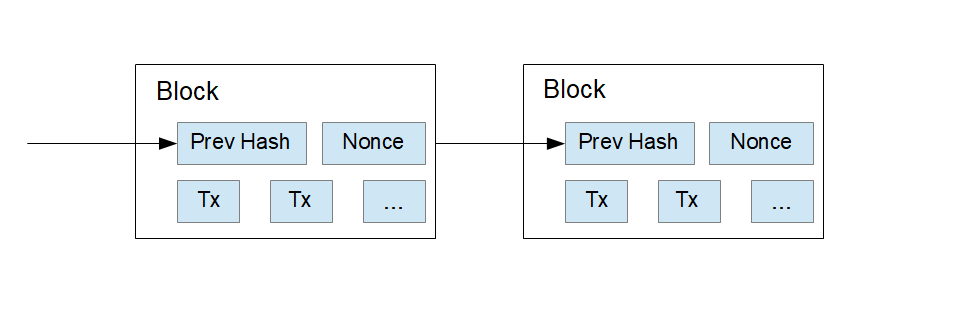
\includegraphics[height=4cm]{blocks}
	\caption{Blocks}
	\label{fig:blocks}
\end{figure}

Beginning with the genesis block, each single block is chained to the previous block by including the the previous hashes. The \ac{SHA-256} takes a 256 bit length of input
messages and hash them to fixed-length outputs \cite{van2014encyclopedia}. So the \ac{SHA-256} function starts by padding the message according to the so-called Merkle-Damg{\aa}rd strengthening technique. Further the message is processed block by block with the the underlying compression function, which initializes an appropriate number of chaining variables to a fixed value to hash the genesis block and also the current hash value for the following blocks \cite{coron2005merkle}. In the year 2003 the \ac{SHA} was published by the \ac{ISO} making \ac{SHA} a standard for most countries in the world \cite{isoSHA-256}. Five years later Satoshi Nakamoto proposed the first concept of a \ac{PoW} based blockchain to allow for public agreement on the order of transactions. The public ethereum blockchain uses \ac{PoW} to this day. There are several other consensus algorithms today suitable for a blockchain and some are considered to be an improvement to \ac{PoW}, which will be discussed later in this work.

\clearpage

\subsection{Ethereum Virtual Machine}
\label{subsec:background:first_section:ethereum}
EXPLAIN ETHEREUM \ac{EVM}

WORLD STATE:
\\
World State. The world state (state), is a mapping
between addresses (160-bit identiers) and account
states (a data structure serialised as RLP, see Appendix
B). Though not stored on the blockchain, it is assumed
that the implementation will maintain this mapping in a
modied Merkle Patricia tree (trie, see Appendix D). The
trie requires a simple database backend that maintains a
mapping of bytearrays to bytearrays; we name this underlying
database the state database. \cite{wood2014ethereum}


- explain how code execution works on a distributed system
 
- explain, that the network can be seen as one comutational resource
- buterin check ethereum code execution \cite{buterin2013ethereum}

%eth vm architecture figure?

\cite{dannen2017introducing}
	%read the evm page 47
%ref to eth paper


\subsection{Smart Contracts}
\label{subsec:background:first_section:first_subsection}
EXPLAIN SMART CONTRACTS HERE 
in ethereum context by wood known simple as contracts
buterin first introduced the term smart contracts
% https://cryptorating.eu/whitepapers/Ethereum/Ethereum_white_paper.pdf
\cite{buterin2013ethereum}
% https://files.gitter.im/ethereum/yellowpaper/VIyt/Paper.pdf
\cite{wood2014ethereum}
% https://solidity.readthedocs.io/en/v0.4.24/introduction-to-smart-contracts.html
% https://link.springer.com/content/pdf/bfm%253A978-1-4842-2535-6%252F1.pdf
\cite{dannen2017introducing}



%\subsection{Assets / Cryptocurrencies (Terminology!!)}
%\label{subsec:background:first_section:third_subsection}
%EXPLAIN ASSETS/CRYPTOS HERE

%\subsection{Public and Private Key (Terminology!!)}
%\label{subsec:background:first_section:fourth_subsection}
%EXPLAIN PUBLIC AND PRIVATE KEYS HERE

\clearpage
%
% Section: Der Zweite Abschnitt
%
\section{Digraphs}
\label{sec:background:second_section}
EXPLAIN DIGRAPHS HERE
\cite{bang2007theory}

\section{Hashlocks and Timelocks}
\label{sec:background:third_section}
EXPLAIN HASH AND TIMELOCKS HERE

%\section{Atomic Transactions (Terminology!!)}
%\label{sec:background:fourth_section}
%EXPLAIN ATOMIC TRANSACTIONS HERE

\section{Atomic Cross-Chain Swaps}
\label{sec:background:fifth_section}

theres also research specifically for ethereum private sidechains \cite{robinson2019atomic}
EXPLAIN ATOMIC CROSS CHAIN SWAPS HERE
\cite{herlihy2018atomic}